
\definecolor{c746c66}{RGB}{116,108,102}


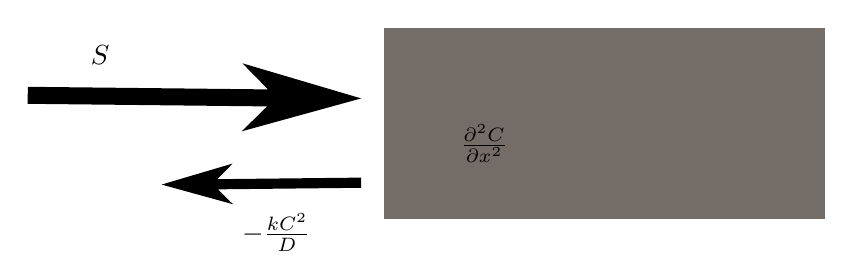
\begin{tikzpicture}[y=0.80pt, x=0.8pt,yscale=-1, inner sep=0pt, outer sep=0pt]
\begin{scope}[shift={(0,-579.86215)}]
  \path[fill=c746c66,line join=miter,line cap=butt,even odd rule,line
    width=1.327pt] (200.9106,774.0675) -- (400.0000,774.0675) --
    (400.0000,860.6569) -- (200.9106,860.6569) -- cycle;
  \path[color=black,fill=black,line join=miter,line cap=butt,miter limit=4.00,even
    odd rule,line width=2.400pt] (136.8727,790.1525) -- (190.5000,806.0161) --
    (136.5876,820.8745) -- (148.0503,809.6270) -- (39.8955,808.4517) --
    (39.9554,800.7699) -- (148.4553,801.9502) -- (136.8726,790.1525) -- cycle;
  \path[fill=black,line join=miter,line cap=butt,line width=0.800pt]
    (68.41143,790.55756) node[above right] (text4542) {$S$};
  \path[fill=black,line join=miter,line cap=butt,line width=0.800pt]
    (235.29883,834.88702) node[above right] (text4986) {$\frac{\partial^{2}
    C}{\partial x^{2}}$};
  \path[color=black,fill=black,line join=miter,line cap=butt,miter limit=4.00,even
    odd rule,line width=2.400pt] (132.4778,835.4371) -- (100.3922,844.9285) --
    (132.6483,853.8184) -- (125.7902,847.0889) -- (190.5000,846.3857) --
    (190.4642,841.7896) -- (125.5479,842.4958) -- (132.4779,835.4371) -- cycle;
  \path[fill=black,line join=miter,line cap=butt,line width=0.800pt]
    (136.73097,875.04431) node[above right] (text5169) {$-\frac{kC^{2}}{D}$};
\end{scope}

\end{tikzpicture}
